\documentclass[11pt,letterpaper,oneside]{article}
\usepackage[T1]{fontenc}
\usepackage[utf8]{inputenc}
\usepackage{lmodern}
\usepackage[margin=0.88in,headheight=16pt,footskip=28pt]{geometry}
\usepackage{microtype}
\usepackage{xcolor}
\usepackage{graphicx}
\usepackage{array,booktabs,longtable,tabularx,multirow}
\usepackage{enumitem}
\usepackage{amssymb,amsmath}
\usepackage{listings}
\usepackage[most]{tcolorbox}
\usepackage{tikz}
\usetikzlibrary{arrows.meta,positioning,shapes.geometric,fit}
\usepackage{titlesec}
\usepackage{fancyhdr}
\usepackage{lastpage}
\usepackage{hyperref}
\usepackage{xurl}
\usepackage{bookmark}
\usepackage{caption}
\usepackage{needspace}
\usepackage{etoolbox}
\definecolor{navy}{HTML}{13263F}
\definecolor{blueaccent}{HTML}{216A9A}
\definecolor{tealaccent}{HTML}{137C83}
\definecolor{muted}{HTML}{526276}
\definecolor{pale}{HTML}{EEF4F8}
\definecolor{lightline}{HTML}{D5E0E8}
\definecolor{codebg}{HTML}{F6F8FA}
\definecolor{warn}{HTML}{A65B14}
\hypersetup{colorlinks=true,linkcolor=navy,urlcolor=blueaccent,citecolor=tealaccent,pdftitle={OpenAI Codex Integration with GitHub Copilot},pdfauthor={Technical Engineering Reference},pdfsubject={Installation, authentication, delegation, security and governance}}
\titleformat{\section}{\Large\bfseries\color{navy}}{\thesection}{0.75em}{}[\vspace{-0.35em}\color{lightline}\titlerule]
\titleformat{\subsection}{\large\bfseries\color{navy}}{\thesubsection}{0.75em}{}
\titleformat{\subsubsection}{\normalsize\bfseries\color{tealaccent}}{\thesubsubsection}{0.6em}{}
\titlespacing*{\section}{0pt}{1.4em}{0.7em}
\titlespacing*{\subsection}{0pt}{1.1em}{0.4em}
\setlist[itemize]{topsep=3pt,itemsep=2pt,parsep=1pt,leftmargin=1.35em}
\setlist[enumerate]{topsep=4pt,itemsep=3pt,parsep=1pt,leftmargin=1.55em}
\renewcommand{\arraystretch}{1.17}
\newcolumntype{Y}{>{\raggedright\arraybackslash}X}
\setlength{\tabcolsep}{5pt}
\setlength{\parskip}{0.32em}
\setlength{\parindent}{0pt}
\pagestyle{fancy}
\fancyhf{}
\fancyhead[L]{\small\color{muted}\textsc{Codex + GitHub Copilot}}
\fancyhead[R]{\small\color{muted}Technical Integration Guide}
\fancyfoot[L]{\small\color{muted}Version 1.0 \textbar\ 16 November 2026}
\fancyfoot[R]{\small\color{muted}\thepage\ / \pageref{LastPage}}
\renewcommand{\headrulewidth}{0.35pt}
\renewcommand{\footrulewidth}{0pt}
\newtcolorbox{infobox}[1][]{colback=pale,colframe=lightline,boxrule=0.5pt,arc=2pt,left=8pt,right=8pt,top=7pt,bottom=7pt,breakable,#1}
\newtcolorbox{riskbox}[1][]{colback=orange!5,colframe=warn!40,boxrule=0.6pt,arc=2pt,left=8pt,right=8pt,top=7pt,bottom=7pt,breakable,#1}
\newcommand{\cmd}[1]{\path{#1}}
\newcommand{\src}[1]{\textsuperscript{\hyperref[ref:#1]{[#1]}}}
\newcommand{\pass}{\textcolor{tealaccent}{\textbf{PASS}}}
\lstdefinestyle{base}{basicstyle=\ttfamily\footnotesize,keywordstyle=\color{navy}\bfseries,commentstyle=\color{muted}\itshape,stringstyle=\color{tealaccent},numbers=left,numberstyle=\tiny\color{muted},numbersep=8pt,breaklines=true,breakatwhitespace=false,frame=single,rulecolor=\color{lightline},backgroundcolor=\color{codebg},showstringspaces=false,tabsize=2,columns=fullflexible,keepspaces=true,postbreak=\mbox{\textcolor{tealaccent}{$\hookrightarrow$}\space},aboveskip=8pt,belowskip=8pt}
\lstdefinestyle{bashstyle}{style=base,language=bash}
\lstdefinestyle{jsonstyle}{style=base,language={}}
\lstdefinestyle{yamlstyle}{style=base,language={}}
\lstdefinestyle{mdstyle}{style=base,language={}}
\lstset{style=base}
\captionsetup{font=small,labelfont={bf,color=navy}}
\newcommand{\key}[1]{\textbf{#1}}
\newcommand{\criterion}[2]{\textbf{#1} & #2\\\hline}
\begin{document}
\hypersetup{pageanchor=false}% unnumbered cover
\begin{titlepage}
\thispagestyle{empty}
\vspace*{1.15in}
{\color{tealaccent}\rule{0.17\linewidth}{3pt}}\\[0.34in]
{\fontsize{29}{34}\selectfont\bfseries\color{navy}OpenAI Codex Integration\\[0.1em] with GitHub Copilot\par}
\vspace{0.24in}
{\Large\color{muted}Architecture, Setup, Delegation, Security, and Enterprise Operations\par}
\vspace{0.48in}
\begin{tcolorbox}[colback=pale,colframe=lightline,boxrule=.5pt,arc=2pt]
\textbf{Scope}\quad GitHub-hosted coding agents; VS Code local and cloud sessions; authentication and billing; permissions and sandboxing; repository instructions; CI/CD; governance; operational troubleshooting.\\[0.28em]
\textbf{Audience}\quad Software engineers, platform engineers, DevSecOps teams, GitHub administrators, and technical reviewers.\\[0.28em]
\textbf{Verification date}\quad 16 November 2026. Features labeled \emph{preview} may change; review vendor documentation before production rollout.
\end{tcolorbox}
\vfill
{\large\bfseries\color{navy}Engineering Technical Reference}\par
{\normalsize\color{muted}Version 1.0 \textbar\ Source-controlled LaTeX / pdfLaTeX compatible}\par
\vspace*{0.65in}
\end{titlepage}\hypersetup{pageanchor=true}
\pagenumbering{roman}
\tableofcontents
\newpage
\pagenumbering{arabic}

\section{Executive Summary and Scope}
GitHub Copilot supports OpenAI Codex as a \emph{third-party coding agent} for delegated software-engineering work. A supported GitHub-hosted task may begin from an issue or prompt and yield changes for review in a pull request. Visual Studio Code (VS Code) can also expose provider-specific Codex sessions, but the local harness, Copilot-hosted cloud experience, and use of a Codex \emph{model} in a different agent harness are not equivalent.\src{GH-AGENTS}\src{VSC-HARNESS}

The most consequential design choice is \emph{where execution occurs and which identity and policy plane controls it}. Cloud delegation relies on GitHub account/repository policies. Local tools may act on the workstation or development container with the permissions allowed by that environment. Production deployment should retain conventional source-control approvals, protected branches, repeatable builds, and audit trails.

\begin{infobox}
\textbf{Status at publication.} GitHub describes third-party coding agents, including Codex, as \emph{public preview}; partner-agent usage draws on AI credits and GitHub Actions minutes. GitHub documentation lists all paid Copilot plans for cloud third-party agents, while \emph{Sign in with Copilot} for the Codex VS Code extension / direct harness integration is restricted to Pro+ and Max. Model catalogs, exact menu labels, and pricing can change independently.\src{GH-AGENTS}\src{VSC-HARNESS}
\end{infobox}

\subsection{In scope and out of scope}
\begin{itemize}
\item \textbf{In scope:} agent selection; installation; account and repository authorization; GitHub issue/PR delegation; local versus managed execution; approval profiles; source instructions; GitHub Actions validation; branch and organization policies; operational controls.
\item \textbf{Out of scope:} undocumented GitHub APIs, guaranteed agent implementation internals, bypassing corporate controls, and claiming that Copilot and Codex share universal cross-provider memory or identical billing.
\end{itemize}

\section{Terminology and Reference Architecture}
\subsection{Four independent dimensions}
\begin{description}[style=nextline,leftmargin=2.9cm,font=\bfseries]
\item[Model] The model producing reasoning or tool requests. Selecting a Codex-family model is not the same as selecting the Codex agent harness.
\item[Agent harness] The runtime that manages tool calls, prompts, permission requests, state and task execution. VS Code distinguishes Copilot, Codex, and other harnesses.\src{VSC-CONCEPT}
\item[Execution target] Local filesystem, Git worktree, remote host, development container, or managed cloud environment. ``Cloud'' describes an execution target, not a guarantee that the local Codex harness is used unchanged.\src{VSC-CONCEPT}
\item[Identity and policy] GitHub Copilot account plus GitHub repository/enterprise controls, or an independent ChatGPT/OpenAI identity depending on selected authentication flow.
\end{description}

\begin{figure}[htbp]
\centering
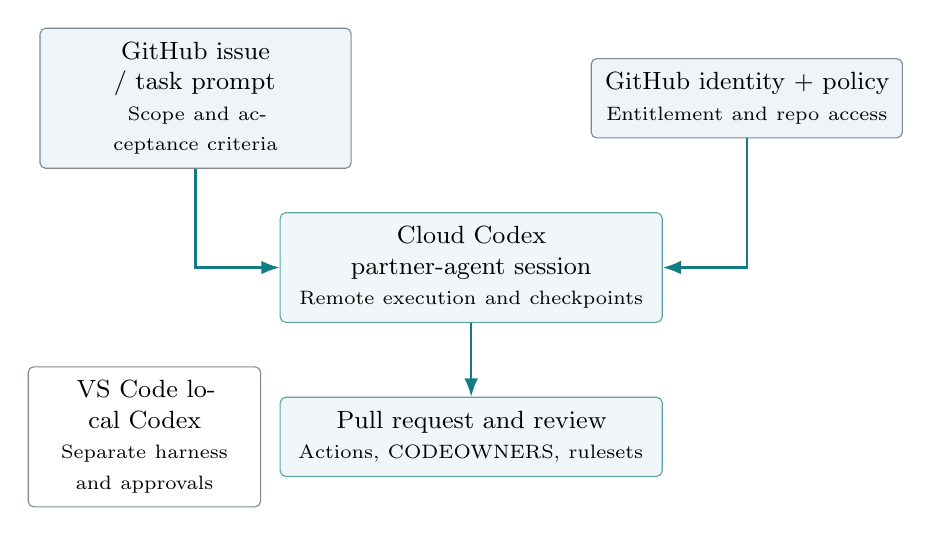
\begin{tikzpicture}[font=\small,>=Latex,
 block/.style={draw=navy!55,rounded corners=2pt,fill=pale,text width=3.6cm,align=center,minimum height=1cm,inner sep=5pt},
 centerblock/.style={draw=tealaccent!70,rounded corners=2pt,fill=tealaccent!6,text width=4.5cm,align=center,minimum height=1.0cm,inner sep=5pt},
 localblock/.style={draw=navy!55,rounded corners=2pt,fill=white,text width=2.6cm,align=center,minimum height=1.05cm,inner sep=5pt}]
\node[block] (issue) at (-3.5,2.8) {GitHub issue / task prompt\\{\scriptsize Scope and acceptance criteria}};
\node[block] (policy) at (3.5,2.8) {GitHub identity + policy\\{\scriptsize Entitlement and repo access}};
\node[centerblock] (cloud) at (0,0.65) {Cloud Codex partner-agent session\\{\scriptsize Remote execution and checkpoints}};
\node[centerblock] (pr) at (0,-1.5) {Pull request and review\\{\scriptsize Actions, CODEOWNERS, rulesets}};
\node[localblock] (local) at (-4.15,-1.5) {VS Code local Codex\\{\scriptsize Separate harness and approvals}};
\draw[->,thick,tealaccent] (issue.south) |- (cloud.west);
\draw[->,thick,tealaccent] (policy.south) |- (cloud.east);
\draw[->,thick,tealaccent] (cloud.south) -- (pr.north);
\end{tikzpicture}
\caption{Conceptual integration and review boundaries. Local and cloud boxes represent distinct run modes with different execution and permission boundaries.}
\end{figure}

\subsection{Choosing a workflow}
\begin{table}[htbp]
\small
\centering
\begin{tabularx}{\linewidth}{@{}>{\raggedright\arraybackslash}p{2.7cm}Y Y@{}}
\toprule
\textbf{Workflow} & \textbf{Best fit} & \textbf{Primary control}\tabularnewline\midrule
GitHub issue delegation & Discrete scoped task; async branch/PR output & GitHub repository policy, PR review and CI\\
GitHub Agents prompt & Investigation or implementation started from a prompt & GitHub session, output review, scope\\
VS Code cloud partner & Hand-off without keeping editor active & Copilot identity, cloud session and policy\\
VS Code local Codex & Iterative refactoring, local builds and editor context & Host sandbox, approvals, workstation hygiene\\
Copilot harness + Codex model & Copilot tools and customizations with selected model & Copilot harness permission model\\
\bottomrule
\end{tabularx}
\caption{Selection matrix. Current support depends on entitlement, version and organization policy.}
\end{table}

\section{Eligibility, Licensing, Usage, and Prerequisites}
\subsection{Plan and identity matrix}
\begin{table}[htbp]
\small
\centering
\begin{tabularx}{\linewidth}{@{}>{\raggedright\arraybackslash}p{3.0cm}>{\raggedright\arraybackslash}p{3.5cm}Y@{}}
\toprule
\textbf{Access path} & \textbf{Documented eligibility} & \textbf{Notes}\tabularnewline\midrule
GitHub cloud third-party coding agents & Paid GitHub Copilot plans & Public preview; repository and policy gates apply.\src{GH-AGENTS}\\
VS Code cloud Codex partner session & Eligible Copilot account and enabled partner agent & OpenAI extension not required for cloud partner sessions.\src{VSC-START}\\
Codex extension: sign in with Copilot & Copilot Pro+ / Max & Copilot-backed models; subject to GitHub limits and billing.\src{GH-AGENTS}\\
VS Code direct Codex Agent Host: GitHub auth & Copilot Pro+ & Experimental or evolving UI.\src{VSC-HARNESS}\\
Codex with ChatGPT sign-in & Eligible ChatGPT identity; see provider entitlements & Independent from a Copilot entitlement; free ChatGPT sign-in may be available for direct Agent Host, subject to limits.\src{VSC-HARNESS}\\
\bottomrule
\end{tabularx}
\end{table}

\begin{riskbox}
\textbf{Billing correction.} Do not use ``one premium request per session'' as a durable cost model. GitHub currently documents consumption of \emph{AI credits according to model and token usage} and GitHub Actions minutes. Configure budgets and review current billing guidance before deployment.\src{GH-AGENTS}
\end{riskbox}

\subsection{Minimum readiness checklist}
\begin{enumerate}
\item Confirm a supported Copilot plan and that the selected login is the entitled GitHub account.
\item Confirm write access to the target GitHub repository; confirm cloud agent access is enabled there.
\item Confirm owner/admin approval for OpenAI Codex under individual, organization and/or enterprise policies.
\item For editor workflows, use a current supported VS Code release with AI features and Copilot configured.
\item For local execution, maintain a clean Git worktree, reproducible build commands, and a least-privilege sandbox.
\item Require human review, checks, and merge protection for any generated source.
\end{enumerate}

\section{Installation and Enablement}
\subsection{Enable GitHub partner agents (personal account)}
\begin{enumerate}
\item Open GitHub Copilot account \emph{cloud agent} settings.
\item Find \textbf{Partner agents}; enable \textbf{OpenAI Codex} if visible and allowed.
\item Navigate to a repository with cloud-agent access, then inspect its \textbf{Agents} entry point or an issue's \textbf{Assignees} menu.
\item If not visible, verify account entitlement, repository policy, organization restrictions and any preview gating.\src{GH-INDIVIDUAL}
\end{enumerate}

\subsection{Enable for organization and enterprise}
\begin{enumerate}
\item \textbf{Enterprise owner:} navigate to \emph{Enterprise $\rightarrow$ AI controls $\rightarrow$ Agents} and permit the relevant agent policies. Enterprise settings may constrain organizations.\src{GH-ENTERPRISE}
\item \textbf{Organization owner:} navigate to \emph{Organization $\rightarrow$ Settings $\rightarrow$ Copilot $\rightarrow$ Cloud agent} (or the current Cloud/partner-agents page) and enable Codex under \emph{Partner agents}.\src{GH-ORG}
\item Scope cloud agent repository access to an approved allowlist, or choose the least-permissive available setting; establish rulesets and reviews for those repositories.\src{GH-CLOUD}
\item Document owners, accepted data categories, billing account, incident contact, and rollback procedure.
\end{enumerate}

\begin{infobox}
GitHub reports that enabling the Codex partner agent installs an associated \texttt{openai code agent} GitHub App; its activity is audit-log visible, although it may not appear in the usual installed GitHub Apps list. Do not confuse this managed partner-agent integration with manually installing an unrelated GitHub Marketplace agent app.\src{GH-AGENTS}
\end{infobox}

\subsection{VS Code: cloud session (without Codex extension)}
\begin{enumerate}
\item Install or update VS Code and authenticate to GitHub Copilot.
\item Ensure the GitHub partner-agent policy permits Codex.
\item Open \emph{Chat $\rightarrow$ New Chat}; select the \textbf{Cloud} session target (UI names may vary).
\item Select \textbf{Codex} from the partner-agent picker; submit a small bounded task.
\item Review the resulting session, branch and pull request, and check CI before merge.\src{VSC-START}
\end{enumerate}

\subsection{VS Code: local extension / direct harness}
\begin{enumerate}
\item In Extensions, search for the \textbf{OpenAI Codex} extension and verify its publisher; install it for extension-based local sessions.
\item Alternatively, on supported VS Code builds, turn on the experimental direct Agent Host integration using \cmd{chat.agentHost.codexAgent.enabled}. This is \emph{not} required by every extension workflow.\src{VSC-HARNESS}
\item Authenticate using the specific supported account flow: \emph{Sign in with Copilot} for eligible Pro+/Max accounts, or an independent \emph{Sign in to ChatGPT} flow where supported.
\item Open a new agent session, choose \textbf{Codex} as the local session/harness target, and select the least-privilege approval preset.
\item Request a \emph{plan-only} first pass on an unfamiliar repository; grant edits only after checking task boundaries.
\end{enumerate}
\begin{lstlisting}[style=jsonstyle,caption={Illustrative VS Code settings.json fragment for supported direct Agent Host builds.}]
{
  "chat.agentHost.codexAgent.enabled": true
}
\end{lstlisting}
\begin{riskbox}
\textbf{Managed settings caveat.} VS Code documents that provider-specific Codex and Claude harnesses may be disabled when enterprise-managed Copilot settings apply, since those harnesses cannot enforce the managed permission/sandbox settings. Having a Codex model available in the Copilot harness does not override that constraint.\src{VSC-CONCEPT}\src{VSC-SECURITY}
\end{riskbox}

\section{Authentication, Authorization, and Trust Boundaries}
\subsection{Authentication paths}
\begin{table}[htbp]
\small
\centering
\begin{tabularx}{\linewidth}{@{}>{\raggedright\arraybackslash}p{3.1cm}Y Y@{}}
\toprule
\textbf{Path} & \textbf{Identity / entitlement} & \textbf{Primary authorization surface}\tabularnewline\midrule
Cloud GitHub agent & GitHub Copilot entitlement & Repository access, GitHub policy, cloud agent permissions\\
Local with Copilot sign-in & GitHub Copilot Pro+/Max & VS Code account, agent approval preset and host rights\\
Local with ChatGPT sign-in & ChatGPT provider account & Provider access plus VS Code/host permissions\\
GitHub Actions validation & \cmd{GITHUB_TOKEN} scoped to workflow & Workflow \cmd{permissions:}, rulesets, runner isolation\\
\bottomrule
\end{tabularx}
\end{table}

Authentication determines \emph{who} can start a session; authorization determines \emph{which repository, tools, files, credentials, and networks} the session may use. These are distinct from branch governance, which determines whether the results may be merged.

\subsection{Required security boundaries}
\begin{itemize}
\item Never paste API tokens, production credentials, private SSH keys, or secrets into prompts, issues, \cmd{AGENTS.md}, logs, or model-generated code.
\item Store authentication in supported account sign-in or credential stores; use ephemeral access credentials where possible.
\item Treat repository content, external documentation, issue comments, and tool output as \emph{untrusted input}; they may contain prompt-injection instructions.
\item Grant network, filesystem, and MCP scope based on task need; disable or restrict deployment tools for coding sessions.
\item Avoid giving local agents broad access to home directories, credential files, production VPN contexts, or shared workstations.
\item Preserve an independent PR review and CI gate even when GitHub performs its agent security scan.
\end{itemize}

\section{Delegating GitHub Issues and Pull Requests}
\subsection{Issue assignment: supported UI workflow}
\begin{enumerate}
\item Create a GitHub issue with context, paths, constraints, acceptance criteria, tests and explicit exclusions.
\item In the issue sidebar, open \textbf{Assignees}. Select \textbf{Codex} if the partner agent is available to the repository and account.
\item Observe progress using the issue timeline, the \textbf{Agents} UI or the session link presented by GitHub.
\item Inspect the resulting changes and pull request; add PR comments mentioning the agent from the GitHub picker to request iteration if supported.
\item Approve after validating tests, security, scope, diff quality and branch rules.\src{GH-AGENTS}
\end{enumerate}

\subsection{Prompt-based and mobile / VS Code entry points}
The repository's \textbf{Agents} tab permits selecting a partner agent and entering a task prompt. GitHub Mobile and VS Code also expose supported task initiation flows. Prompt-started sessions and issue-started sessions need not have identical branch/PR behavior; check the current flow's UI rather than assuming that every prompt immediately opens a draft PR.\src{GH-AGENTS}\src{GH-KICKOFF}

\begin{riskbox}
\textbf{Avoid undocumented CLI shortcuts.} A human-readable agent option in the GitHub Assignees UI is not proof that \cmd{gh issue edit N --add-assignee "@codex"} is accepted as a normal user login across all repositories. The supported UI path is the baseline; automate assignment only against a documented and tested API or CLI integration for your environment.
\end{riskbox}

\subsection{Example: issue template}
\begin{lstlisting}[style=mdstyle,caption={Recommended GitHub issue body; replace paths and checks.}]
## Objective
Add a focused integration guide for Codex and GitHub Copilot.

## Scope
- Create one self-contained pdfLaTeX-compatible .tex source.
- Follow current repository structure and documentation style.
- Add no new network, deployment, or credential dependencies.

## Non-goals
- Do not refactor unrelated documents or workflows.
- Do not modify protected branch settings or CI secrets.

## Acceptance criteria
- [ ] The document builds with pdflatex / latexmk.
- [ ] Hyperlinks and references resolve.
- [ ] make preflight succeeds in the repository.
- [ ] Only approved files appear in the pull request diff.
- [ ] Existing CI checks pass; a human reviewer approves.

## Evidence requested
Record commands executed, output path, test results, and
limitations / assumptions in the pull request description.
\end{lstlisting}

\subsection{Example: delegation prompt}
\begin{lstlisting}[style=mdstyle,caption={Bounded delegation with reviewable deliverables.}]
Read README.md, Makefile, .latexmkrc and relevant AGENTS.md
instructions before editing. Implement only the linked issue.

Plan first. Name files to change and explain dependencies.
Do not add packages, change publishing workflows, or alter
security configuration without human approval.

After implementation:
1. Run project preflight and targeted build validation.
2. Inspect warnings, links, tables, and code listings.
3. Run git diff --check and list changed files.
4. Open or update the PR with evidence and open questions.
5. Do not merge, deploy, or dismiss security alerts.
\end{lstlisting}

\section{Local Versus Cloud Execution}
\subsection{Execution and isolation semantics}
\begin{table}[htbp]
\small
\centering
\begin{tabularx}{\linewidth}{@{}>{\raggedright\arraybackslash}p{2.65cm}Y Y@{}}
\toprule
\textbf{Dimension} & \textbf{Local Codex} & \textbf{GitHub-managed cloud Codex}\tabularnewline\midrule
Workspace & Local repository/worktree, remote WSL or dev container & Session-managed repository branch/environment\\
Tool execution & Host-access boundaries; filesystem & Remote compute and configured tools\\
Credentials & Local provider login; host stores & GitHub account, repo permissions, managed session\\
Network & Per local approval/sandbox policy & Managed environment; policy-dependent\\
Continuity & Usually interactive through editor & Supports asynchronous delegated work\\
Output & Local modified files/commits & Changes for PR review\\
Risk & Local credential, filesystem and network exposure & Repository content, execution supply chain, permissions, PR trust\\
\bottomrule
\end{tabularx}
\end{table}

\subsection{Selection decision tree}
\begin{enumerate}
\item Is the task self-contained with explicit acceptance criteria and a clean PR-based review process? Prefer \textbf{cloud issue delegation}.
\item Does it depend on a local debugger, hardware, private development environment or live interactive feedback? Prefer \textbf{local Codex} in a restricted worktree or dev container.
\item Must enterprise-managed Copilot restrictions apply uniformly? Prefer the \textbf{Copilot harness} and approved models; check whether provider-specific harnesses are disabled.
\item Does the task touch privileged infrastructure, production data or sensitive secrets? Use a separate approved automation design and human approval; do not elevate a general-purpose coding agent by default.
\end{enumerate}

\section{Permission Modes, Approval Presets, and Sandboxing}
\subsection{Direct Codex Agent Host presets}
VS Code describes the following \emph{direct Codex integration} permission presets; extension-specific behavior can differ and must be checked against the extension's documentation.\src{VSC-APPROVAL}
\begin{table}[htbp]
\small
\centering
\begin{tabularx}{\linewidth}{@{}>{\raggedright\arraybackslash}p{2.8cm}Y >{\raggedright\arraybackslash}p{3.3cm}@{}}
\toprule
\textbf{Preset} & \textbf{Behavior documented by VS Code} & \textbf{Recommended usage}\tabularnewline\midrule
Default Permissions & Read/edit workspace, routine commands; requests approval for network and outside-workspace access & Default for normal development\\
Auto-Review & Same workspace access; automatic reviewer handles approval requests & Restricted workspaces after policy review\\
Full Access & Broader disk and network access without asking & Exceptional isolated contexts only\\
\bottomrule
\end{tabularx}
\end{table}

\begin{riskbox}
\textbf{Full Access is not a productivity default.} It allows unrestricted disk and network access. VS Code also offers global auto-approval options that suppress prompts across workspaces. Neither is an appropriate general-purpose enterprise standard. Avoid \cmd{/yolo}, global auto-approve, or similar bypasses in production-connected environments.\src{VSC-APPROVAL}
\end{riskbox}

\subsection{Review policy for operations}
\begin{itemize}
\item \textbf{Read-only investigation:} accept file reads and bounded search; deny writes unless scope changes.
\item \textbf{Contained workspace edits:} allow edits inside the checked-out worktree, then inspect diff.
\item \textbf{Dependency installation / internet:} require approval and verified provenance. Pin versions and document added dependencies.
\item \textbf{Outside workspace access / shell escalation:} deny by default; use a dedicated container when necessary.
\item \textbf{Git remote writes / PR operations:} require authenticated user intent and normal branch policies; block unattended merges.
\item \textbf{Infrastructure changes or secrets:} handle via separate change-control and production deployment authorization.
\end{itemize}

\subsection{Defense in depth}
An effective implementation couples least privilege, isolation, allowlisted networks, disposable credentials, commit review, automated checks, secret scanning, and human approval. Runtime approval prompts are a \emph{single} layer, not a security guarantee. VS Code security guidance highlights worktree isolation and secure handling of MCP credentials, while explicitly cautioning that provider harnesses may not enforce managed Copilot settings.\src{VSC-SECURITY}

\section{Repository Instructions: AGENTS.md and Related Files}
\subsection{Role and instruction hierarchy}
\cmd{AGENTS.md} supplies standing guidance to AI coding agents: repository orientation, ownership, coding conventions, test/build commands, change boundaries and validation expectations. It is \emph{instruction text, not a permission enforcement mechanism}. Provider-specific discovery and precedence may vary; OpenAI documents root-to-leaf inheritance for its own Codex tooling.\src{OPENAI-AGENTS}

In a GitHub repository, distinguish:
\begin{itemize}
\item \cmd{AGENTS.md}: cross-agent repository operating instructions.
\item \cmd{.github/copilot-instructions.md}: Copilot-specific global instructions, especially useful for Copilot code review.
\item \cmd{.github/instructions/*.instructions.md}: path-scoped Copilot review instructions.
\item \cmd{.github/skills/}: focused agent skills or workflows, where supported.\src{GH-REVIEW}
\end{itemize}

\subsection{Complete example for a LaTeX documentation repository}
The following illustrative root file is tailored to a repository whose source roots live under \cmd{src/} and whose authoritative build is driven by \cmd{Makefile}. Validate the actual repository instructions before committing.
\begin{lstlisting}[style=mdstyle,caption={Example AGENTS.md; repository-level guidance is advisory, not a security policy.}]
# AGENTS.md - LaTeX documentation engineering

## Repository contract
- LaTeX source under src/ is authoritative.
- PDFs are generated artifacts; avoid committing them unless
  the repository's publishing policy requires it.
- Prefer pdfLaTeX-compatible packages and syntax.
- Do not introduce minted or shell escape without approval.
- Preserve existing document structure and source links.

## Before editing
1. Read README.md, Makefile and .latexmkrc.
2. Inspect the relevant neighboring .tex files.
3. Identify document root vs included fragments.
4. State the proposed file changes and unresolved assumptions.

## Implementation rules
- Use T1 font encoding, UTF-8 input and stable hyperlinks.
- Prefer listings with line numbers, wrapping, and framed code.
- Keep tables within margins; use tabularx/longtable if needed.
- Keep content sourced; mark changing vendor behavior as such.
- Do not edit unrelated files, CI, secrets, or deployment config.

## Validation
- Run: make preflight
- Run: latexmk -pdf -interaction=nonstopmode \
       -halt-on-error path/to/document.tex
- Inspect PDF for clipping, broken links and missing glyphs.
- Run: git diff --check
- Record checks and changed files in the PR.

## Safety and review
- Never place credentials, tokens or private data in sources.
- Do not merge PRs, bypass branch rules, dismiss alerts,
  modify CODEOWNERS or approve your own changes.
- Stop and request a reviewer if tasks exceed approved scope.
\end{lstlisting}

\subsection{Optional path-specific instructions}
\begin{lstlisting}[style=mdstyle,caption={Example src/devops/AGENTS.md for more specific local instructions.}]
# DevOps documentation supplement

- Use verified vendor documentation for versioned settings.
- Differentiate preview, generally available and deprecated
  functionality explicitly.
- Include threat boundaries, failure modes and rollback steps.
- Keep example GitHub Actions token permissions minimal.
\end{lstlisting}

\subsection{Governance of instructions}
Require review for changes to \cmd{AGENTS.md}, \cmd{CODEOWNERS}, workflows, settings, permission documentation and security controls. Maintain a named owner for each instruction file, and ensure technical assertions can be validated. A malicious pull request could modify instructions to tell an agent to ignore safety or leak data; review instruction diffs as security-relevant changes.

\section{CI/CD Integration and GitHub Actions}
\subsection{Separation of responsibilities}
The agent may produce code and propose changes, but \emph{CI verifies} and \emph{humans authorize promotion}. The standard path is issue $\rightarrow$ agent branch $\rightarrow$ PR $\rightarrow$ static checks / tests / security review $\rightarrow$ code-owner approval $\rightarrow$ protected-branch merge $\rightarrow$ separately authorized deployment. Do not treat agent-generated tests as independent proof that the implementation is safe.

\subsection{Minimum PR validation workflow}
The following example demonstrates an isolated, read-only validation job for a single stand-alone \LaTeX\ file. It is a \emph{reference template}, not a replacement for an existing repository's build/publish workflows. Adjust package installation and document path to your environment.
\begin{lstlisting}[style=yamlstyle,caption={.github/workflows/codex-latex-validation.yml -- read-only PR validation.}]
name: Codex LaTeX validation

on:
  pull_request:
    paths:
      - 'src/**/*.tex'
      - 'AGENTS.md'
      - '.github/workflows/codex-latex-validation.yml'
  workflow_dispatch:

permissions:
  contents: read

jobs:
  latex-check:
    runs-on: ubuntu-latest
    timeout-minutes: 20
    steps:
      - name: Check out repository
        uses: actions/checkout@v4
        with:
          fetch-depth: 0
      - name: Install LaTeX toolchain
        run: |
          sudo apt-get update
          sudo apt-get install -y --no-install-recommends \
            latexmk texlive-latex-base texlive-latex-recommended \
            texlive-latex-extra texlive-fonts-recommended
      - name: Repository preflight
        run: make preflight
      - name: Compile integration guide
        run: |
          latexmk -pdf -interaction=nonstopmode -halt-on-error \
            src/devops/ai-agents/codex-github-copilot-integration.tex
      - name: Check whitespace in PR diff
        run: git diff --check "origin/${{ github.base_ref }}...HEAD"
\end{lstlisting}

\begin{infobox}
\textbf{Production integration.} A repository with a mature Makefile/build planner should generally extend its existing changed-document build and checks rather than introducing a parallel pipeline. For \cmd{latex-docs}, review \cmd{make preflight}, \cmd{make build-changed}, its actual workflow files and published PDF coverage before adopting the example above. The sample document path is a \emph{proposed location}, not a claim that the file already exists.
\end{infobox}

\subsection{Recommended branch and repository protection}
\begin{enumerate}
\item Protect \cmd{main} with a ruleset: no direct pushes, required status checks, and at least one independent review (more for sensitive projects).
\item Use \cmd{CODEOWNERS} for critical agent instructions, workflows, security docs and deployment configurations; make code-owner review mandatory.
\item Restrict \cmd{GITHUB_TOKEN} via workflow/job \cmd{permissions:}; prefer \cmd{contents: read} for PR checks.
\item Use environment protection and short-lived OIDC credentials for deployments, in a separate trusted workflow.
\item Pin third-party actions by reviewed full commit SHA in a hardened production pipeline; upgrade under controlled dependency updates.
\item Scan dependencies and secrets in CI; monitor alerts, but do not automatically dismiss findings merely because the PR originated from an agent.
\end{enumerate}

\subsection{Threat model for automation}
\begin{table}[htbp]
\small
\centering
\begin{tabularx}{\linewidth}{@{}>{\raggedright\arraybackslash}p{2.45cm}Y Y@{}}
\toprule
\textbf{Threat} & \textbf{Example failure} & \textbf{Mitigation}\tabularnewline\midrule
Prompt injection & Issue text attempts to override restrictions & Treat prompt/context as untrusted; review edits and approvals\\
Secret exfiltration & Task attempts credential read or network POST & Worktree/sandbox restrictions; no secrets in agent context\\
Supply chain & Added unvetted action or dependency & Dependency policy, pinning, reviews, vulnerability scanning\\
Workflow privilege & Unsafe \cmd{pull_request_target} checks out attacker code & Use unprivileged PR workflow; isolate trusted release flow\\
Policy bypass & Agent edits its own instructions or CI requirements & Protect instructions/workflows with review rulesets\\
Silent bad changes & Tests pass but implementation changes unrelated behavior & Scope checks, reviewers, regression tests, diff inspection\\
\bottomrule
\end{tabularx}
\end{table}

GitHub specifically cautions that \cmd{pull_request_target} jobs can carry elevated repository trust; do not execute untrusted PR code with that event's privileged token or secrets.\src{GH-PR-TARGET}

\subsection{Agent security scans are supplemental}
GitHub documents automatic validation of third-party coding-agent changes using CodeQL, secret scanning and dependency advisory data before finalizing output. These checks reduce risk but do \emph{not} guarantee absence of vulnerabilities and are not substitutes for required organization scans, test coverage, independent review or deployment approval.\src{GH-AGENTS}

\section{Enterprise Governance Operating Model}
\subsection{Control plane and ownership}
\begin{table}[htbp]
\small
\centering
\begin{tabularx}{\linewidth}{@{}>{\raggedright\arraybackslash}p{3.0cm}Y >{\raggedright\arraybackslash}p{2.3cm}@{}}
\toprule
\textbf{Control} & \textbf{Policy intent / evidence} & \textbf{Primary owner}\tabularnewline\midrule
Agent entitlement & Approved account and model/agent availability & Enterprise AI admin\\
Repository allowlist & Approved repositories for cloud delegation & Org/repo owner\\
Data classification & Permitted content classes and retention review & Security / legal\\
Permission baseline & No default full-access mode; sandboxed workspaces & Endpoint / platform\\
Network/MCP access & Reviewed tool integrations and allowlists & Platform security\\
Merge governance & Branch rules, status checks and human review & Repository owner\\
Cost limits & Budgets, AI credit and Actions-minute review & FinOps / platform\\
Incident response & Audit events, secret rotation and containment & Security operations\\
\bottomrule
\end{tabularx}
\end{table}

\subsection{Deployment policy tiers}
\begin{description}[style=nextline,leftmargin=1.5em,font=\bfseries]
\item[Tier 0 --- experimentation.] Approved test repositories, synthetic data, local restricted sessions, no production secrets. Human review for all merges.
\item[Tier 1 --- routine engineering.] Named teams and repositories, documented instructions, read-only CI, CodeQL/secret scanning and required checks.
\item[Tier 2 --- high-impact repositories.] Enhanced code-owner approvals, data assessment, network restrictions, preapproved dependencies, detailed audit retention and deployment isolation.
\item[Tier 3 --- privileged operations.] No autonomous access by default. Separate change tickets, privileged identity controls, explicit approvals and production-specific runbooks.
\end{description}

\subsection{Audit, cost, and data controls}
\begin{itemize}
\item Record \emph{who} delegated, \emph{what} issue or prompt initiated work, \emph{where} files changed, and \emph{which} reviews/checks permitted merge.
\item Check the GitHub audit log for agent-app operations and policy changes. Partner-agent Apps can be audit-visible without appearing in the normal app installation list.\src{GH-AGENTS}
\item Monitor AI credits, model/token consumption and GitHub Actions minutes; set budget thresholds and team usage reviews.\src{GH-AGENTS}
\item Align data retention, geographical/regulatory constraints, intellectual-property review, source classification and approved model-provider access with enterprise policy; do not infer them from marketing wording such as ``shared context''.
\item Establish a kill switch: disable partner-agent policy, suspend repository cloud agent access, revoke relevant local sessions/tokens, and quarantine suspicious PRs.
\end{itemize}

\subsection{Responsibility assignment (RACI-style)}
\begin{table}[htbp]
\small
\centering
\begin{tabularx}{\linewidth}{@{}>{\raggedright\arraybackslash}p{3.35cm}>{\raggedright\arraybackslash}p{2.3cm}>{\raggedright\arraybackslash}p{2.3cm}Y@{}}
\toprule
\textbf{Activity} & \textbf{Accountable} & \textbf{Responsible} & \textbf{Consulted}\tabularnewline\midrule
Enterprise enablement & Enterprise AI owner & Enterprise admin & Security, legal\\
Repository onboarding & Repository owner & Platform engineering & Engineering lead\\
Agent instruction review & Engineering lead & Repo maintainer & AppSec\\
Issue delegation & Task owner & Authorized engineer & Reviewer\\
PR merge authorization & Repository owner & Independent reviewer & CI / AppSec\\
Billing and utilization & Platform owner & FinOps & Organization admin\\
Incident containment & Security incident commander & SecOps & Repository owner\\
\bottomrule
\end{tabularx}
\end{table}

\section{Troubleshooting and Diagnostic Runbooks}
\subsection{Symptom-to-cause matrix}
\begin{longtable}{@{}>{\raggedright\arraybackslash}p{3.25cm}>{\raggedright\arraybackslash}p{4.7cm}>{\raggedright\arraybackslash}p{5.0cm}@{}}
\toprule
\textbf{Symptom} & \textbf{Likely cause / checks} & \textbf{Corrective action}\tabularnewline\midrule\endhead
Codex missing from issue Assignees & Paid Copilot plan absent; partner toggle disabled; org/enterprise deny; repo not enabled; UI rollout & Verify account, enterprise/organization/individual policy, repo eligibility; refresh page.\\
Codex missing from VS Code cloud picker & Wrong session target, GitHub account, policy or editor version & Update VS Code, reauthenticate GitHub, choose Cloud then partner agent; verify GitHub policy.\\
Local Codex option missing & OpenAI extension not installed, direct integration disabled, unsupported build & Install verified extension or supported direct harness; reload window.\\
Copilot sign-in unavailable & Pro+/Max requirement for extension, wrong GitHub account & Verify subscription and current sign-in; consider supported ChatGPT sign-in if appropriate.\\
Local harness disabled by enterprise settings & Managed permission/sandbox policy may be incompatible & Use approved Copilot harness; ask IT/admin before changing policy.\\
Approval prompts too frequent & Default permissions correctly block network/outside workspace access & Use documented dependency mirrors, preapproved isolated dev container; do not set Full Access by default.\\
Agent claims success but PR checks fail & Missing dependency, incorrect path, syntax/build regression & Inspect CI logs, reproduce command, request bounded repair.\\
Build fails on LaTeX source & Missing package, non-pdfLaTeX syntax, unknown code-listing style, broken refs & Run \cmd{make preflight}, targeted \cmd{latexmk}; inspect first compiler error and PDF render.\\
Unexpected file modifications & Scope drift or malicious instructions in context & Stop session, inspect \cmd{git diff}, revert unrelated files, re-evaluate trust.\\
Secret found in PR & Accidental credential disclosure & Block merge, revoke/rotate secret, purge per incident process, inspect audit events.\\
Missing issue/agent activity & Session not initialized; unsupported client; permissions; preview limit & Inspect issue timeline / Agents session UI; verify account and billing/usage dashboard.\\
Unexpected cost spike & Large tool/context loops, repeated sessions, lengthy builds & Review AI credits/actions minutes, narrow task and timeouts, enforce budgets.\\
\bottomrule
\end{longtable}

\subsection{Safe diagnostic commands}
These commands inspect local repository state and validation only. They do not assign a GitHub agent, elevate its permissions, or authorize merges.
\begin{lstlisting}[style=bashstyle,caption={Local read-only/validation diagnostics.}]
git status --short
git diff --stat
git diff --check
git remote -v
make help
make preflight
latexmk -pdf -interaction=nonstopmode -halt-on-error \
  path/to/document.tex
\end{lstlisting}

\subsection{Incident response for suspicious agent behavior}
\begin{enumerate}
\item Stop the agent session and refrain from approving additional tool requests.
\item Disable partner-agent access at the appropriate policy level if a systemic issue is suspected.
\item Preserve issue/PR URLs, audit events, changed files, action logs and relevant timestamps.
\item Revoke/rotate exposed credentials; identify outbound integrations and affected repositories.
\item Block affected PRs and temporarily restrict merge permissions where necessary.
\item Investigate root cause: user instruction, repository prompt injection, dependency provenance, permission misconfiguration or workflow privilege.
\item Restore from clean commit and tested configuration, then document follow-up controls.
\end{enumerate}

\section{Implementation Playbook and Measurable Acceptance Criteria}
\subsection{Thirty-day rollout example}
\begin{enumerate}[label=\textbf{Phase \arabic*.}]
\item \textbf{Policy and design (days 1--5).} Select repository pilots, confirm enterprise and user entitlements, classify data, define review roles, document billing and permissible tool scopes.
\item \textbf{Restricted pilot (days 6--12).} Enable Codex for low-risk repositories; validate local/cloud sign-in, issue delegation, builds, and rollback.
\item \textbf{Engineering controls (days 13--20).} Add \cmd{AGENTS.md}, status checks, source scanning, workflow permission hardening, CODEOWNERS and audit review.
\item \textbf{Operational readiness (days 21--30).} Perform tabletop test, review quality metrics, document support runbook and expand only upon approved evidence.
\end{enumerate}

\subsection{Acceptance test matrix}
\small
\begin{longtable}{@{}>{\raggedright\arraybackslash}p{1.45cm}>{\raggedright\arraybackslash}p{4.35cm}>{\raggedright\arraybackslash}p{6.9cm}@{}}
\toprule
\textbf{ID} & \textbf{Criterion} & \textbf{Evidence / pass condition}\tabularnewline\midrule\endhead
A-01 & Entitlement and policy & A designated owner documents eligible plan; partner-agent toggle; repository allowlist; policy hierarchy.\\
A-02 & Cloud delegation & One approved test issue starts a Codex session; output is traceable to a branch/PR and issue.\\
A-03 & Authentication isolation & Authorized user can sign in; unapproved or wrong-account path cannot access pilot repository.\\
A-04 & Local permission baseline & Default or more restrictive preset demonstrated; outside-workspace/network request prompts or is denied.\\
A-05 & Build reproducibility & \cmd{make preflight} and a clean targeted \cmd{latexmk} build return exit code zero.\\
A-06 & Source quality & No unresolved references, missing figures, clipped tables or unrendered listing text in reviewed PDF.\\
A-07 & Minimal privilege CI & PR workflow grants only read permissions; no unnecessary secrets; trusted deployment separated.\\
A-08 & Branch governance & Direct push to protected branch denied; required CI and independent PR approval enforced.\\
A-09 & Instruction integrity & \cmd{AGENTS.md} and sensitive workflows are subject to mandatory review or rulesets.\\
A-10 & Scanning and triage & Code/secret/dependency scan evidence reviewed; unresolved High/Critical findings escalated to policy owner.\\
A-11 & Audit and cost visibility & Admin can locate session/policy events and usage reports, including Actions minutes and AI credits.\\
A-12 & Incident drill & Test team can disable agent use, block merge, preserve evidence and revoke simulated credential.\\
\bottomrule
\end{longtable}
\normalsize

\subsection{Quality and efficiency metrics}
Track pilot metrics with explicit numerators/denominators and a human-reviewed baseline:
\begin{itemize}
\item \textbf{First-pass CI success rate:} agent-origin PRs passing required checks on first run divided by total agent-origin PRs.
\item \textbf{Rework fraction:} agent-origin PRs requiring a human-requested substantive rework divided by agent-origin PRs reviewed.
\item \textbf{Merge lead time:} median time from agent task submission to reviewed merge; compare only similarly scoped issues.
\item \textbf{Security escape rate:} confirmed post-merge security defects attributable to agent-origin changes per reviewed merged PR.
\item \textbf{Unit economics:} AI credits plus Actions compute per accepted change; separate infrastructure from model consumption.
\item \textbf{Policy exceptions:} number of Full Access / global approval bypasses and reviewed justifications; target zero in general-purpose environments.
\end{itemize}

\section{Applied Example for the \texttt{latex-docs} Repository}
The repository's published README identifies \cmd{src/} as its domain-organized document tree, \cmd{Makefile} and \cmd{tooling/scripts/latex_build.py} as its build facade, and a \emph{pdfLaTeX-only} preflight policy. PDFs are build products, whereas LaTeX source is authoritative.\src{REPO-README}

The canonical source for this guide is \cmd{src/data-systems/ai-agent-engineering/technical-documents/codex-github-copilot-integration-guide.tex}, alongside the related agent harness, Codex subagent, and \cmd{AGENTS.md} references. The AI Agent Engineering navigation and semantic catalogs index this source; DevOps documentation links to it rather than copying it.

\begin{lstlisting}[style=bashstyle,caption={Local build and catalog validation for the canonical source.}]
# From the latex-docs repository root after integration:
make preflight
python3 tooling/scripts/build_semantic_catalogs.py --check
cd src/data-systems/ai-agent-engineering/technical-documents
latexmk -pdf -interaction=nonstopmode -halt-on-error \
  codex-github-copilot-integration-guide.tex
cd ../../../..
git diff --check
git status --short
\end{lstlisting}

For subsequent updates, regenerate the semantic catalog indexes as documented in \cmd{catalog/README.md}, and run the existing changed-root validation workflow. Review source diffs and rendered PDF output before merging to the default branch.

\section{Common Misconceptions and Verification Notes}
\begin{enumerate}
\item \textbf{``Codex uses the same shared memory as Copilot and Claude.''} No general shared cross-agent memory guarantee is established by the cited documentation. Tool, session and context integrations differ.
\item \textbf{``Any paid Copilot plan unlocks local Codex login.''} Cloud partner-agent plan eligibility differs from the Pro+/Max Copilot-login requirement for local Codex integration.
\item \textbf{``The Codex model and harness are interchangeable.''} They are different layers; choosing a model does not switch the harness.\src{VSC-CONCEPT}
\item \textbf{``A GitHub issue can always be assigned with a literal \cmd{@codex} CLI username.''} The UI supports partner-agent assignment; ordinary user-assignable login behavior should not be presumed or scripted without verification.
\item \textbf{``Agent checks eliminate human review.''} Automated scanning is supplemental to branch rules, CI and independent approvals.
\item \textbf{``A preview menu path is permanent.''} Features, client UI and model catalogs change. Verify against source register when updating this document.
\end{enumerate}

\section{Maintenance and Change-Control Checklist}
\begin{itemize}
\item \textbf{Monthly:} recheck preview/GA/deprecation notices, model and plan requirements, partner agent enablement paths, billing basis, and permission presets.
\item \textbf{Quarterly:} audit enabled repositories, code-owner protection, agent-origin PR metrics, policies and network/MCP integrations.
\item \textbf{On incident or major release:} validate threat model, credential boundaries, workflow semantics and documented recovery steps.
\item \textbf{After every guide edit:} recompile with pdfLaTeX, inspect output, validate hyperlinks, and update the source register and verification date.
\end{itemize}

\appendix
\section{One-Page Administrator Checklist}
\begin{itemize}[label=$\square$]
\item Confirm organization/enterprise Copilot subscription and partner-agent policies.
\item Confirm GitHub cloud agent repository scope and agent-specific access.
\item Document eligible user authentication paths and account ownership.
\item Approve bounded pilot repositories and permitted data classifications.
\item Prohibit unconditional Full Access and global tool auto-approval.
\item Protect \cmd{main}, \cmd{AGENTS.md}, workflows and \cmd{CODEOWNERS}.
\item Require human review plus successful security/test/build checks.
\item Monitor AI credits, Actions minutes, audit events, and model/provider updates.
\item Run a stop-session / secret-rotation / disable-access tabletop exercise.
\item Establish a quarterly documentation verification cycle.
\end{itemize}

\section{Source Register and Verification Basis}
\small
Official vendor documentation forms the primary source of product-behavior claims. Repository facts are based on the connected GitHub repository's README and Makefile inspected on 16 November 2026. Sample configurations are illustrative engineering recommendations and are not represented as vendor guarantees.

\begin{description}[style=nextline,leftmargin=1.6cm,font=\bfseries]
\item[GH-AGENTS]\phantomsection\label{ref:GH-AGENTS} GitHub, \emph{Third-party coding agents}.\par\url{https://docs.github.com/en/copilot/concepts/agent-capabilities/about-agents/about-third-party-coding-agents}
\item[GH-INDIVIDUAL]\phantomsection\label{ref:GH-INDIVIDUAL} GitHub, \emph{Managing GitHub Copilot policies as an individual subscriber}.\par\url{https://docs.github.com/en/copilot/how-tos/manage-your-account/manage-policies}
\item[GH-ORG]\phantomsection\label{ref:GH-ORG} GitHub, \emph{Managing policies and features for GitHub Copilot in your organization}.\par\url{https://docs.github.com/en/copilot/how-tos/administer-copilot/manage-for-organization/manage-policies}
\item[GH-ENTERPRISE]\phantomsection\label{ref:GH-ENTERPRISE} GitHub, \emph{Managing policies and features for GitHub Copilot in your enterprise}.\par\url{https://docs.github.com/en/enterprise-cloud@latest/copilot/how-tos/administer-copilot/manage-for-enterprise/manage-enterprise-policies}
\item[GH-CLOUD]\phantomsection\label{ref:GH-CLOUD} GitHub, \emph{Managing GitHub Copilot in the cloud for your organization}.\par\url{https://docs.github.com/en/copilot/how-tos/administer-copilot/manage-for-organization/manage-copilot-in-the-cloud}
\item[GH-KICKOFF]\phantomsection\label{ref:GH-KICKOFF} GitHub, \emph{Kick off a task with Copilot agents on GitHub}.\par\url{https://docs.github.com/en/copilot/how-tos/copilot-on-github/use-copilot-agents/kick-off-a-task}
\item[GH-REVIEW]\phantomsection\label{ref:GH-REVIEW} GitHub, \emph{Using GitHub Copilot code review}.\par\url{https://docs.github.com/en/copilot/how-tos/use-copilot-agents/use-code-review}
\item[GH-PR-TARGET]\phantomsection\label{ref:GH-PR-TARGET} GitHub, \emph{Securely using pull\_request\_target}.\par\url{https://docs.github.com/en/actions/reference/security/securely-using-pull_request_target}
\item[VSC-START]\phantomsection\label{ref:VSC-START} VS Code, \emph{Using third-party agents in VS Code}.\par\url{https://code.visualstudio.com/learn/agents/4-using-third-party-agents-in-vs-code}
\item[VSC-HARNESS]\phantomsection\label{ref:VSC-HARNESS} VS Code, \emph{Choose an agent harness}.\par\url{https://code.visualstudio.com/docs/agents/run/agent-harnesses}
\item[VSC-CONCEPT]\phantomsection\label{ref:VSC-CONCEPT} VS Code, \emph{Understand agent harnesses}.\par\url{https://code.visualstudio.com/docs/agents/concepts/agent-harnesses}
\item[VSC-APPROVAL]\phantomsection\label{ref:VSC-APPROVAL} VS Code, \emph{Manage approvals and permissions}.\par\url{https://code.visualstudio.com/docs/agents/run/approvals}
\item[VSC-SECURITY]\phantomsection\label{ref:VSC-SECURITY} VS Code, \emph{Secure AI-assisted development in VS Code}.\par\url{https://code.visualstudio.com/docs/agents/run/security}
\item[OPENAI-AGENTS]\phantomsection\label{ref:OPENAI-AGENTS} OpenAI, \emph{Custom instructions with AGENTS.md}.\par\url{https://learn.chatgpt.com/docs/agent-configuration/agents-md}
\item[REPO-README]\phantomsection\label{ref:REPO-README} \cmd{Notoriousjayy/latex-docs}, \emph{README.md; Makefile}.\par\url{https://github.com/Notoriousjayy/latex-docs}
\end{description}

\vspace{1em}
\begin{infobox}
\textbf{Maintenance note.} This reference is a dated technical guide, not a dynamic policy engine. Confirm current product UI and published entitlement, security, and billing rules before operational changes.
\end{infobox}
\end{document}
